\documentclass[12pt]{article}

\title{\vspace{-3em}PHYS 202a HW 6}
\author{Michael Cardiff}
\date{\today}

%% science symbols 
\usepackage{amssymb,amsthm,bm,physics,slashed,tikz-feynhand}

%% general pretty stuff
\usepackage{hyperref,caption,enumitem,float,geometry,graphicx,tikz}

% setups
\graphicspath{ {./figs/} }
\captionsetup{labelfont=bf}
\geometry{margin=1in}

% macros
\renewcommand{\L}{\mathcal{L}}
\newcommand{\D}{\partial}
\newcommand{\veps}{\varepsilon}
\newcommand{\circled}[1]{\tikz[baseline=(char.base)]{
    \node[shape=circle,draw,inner sep=2pt](char){#1};}}

\def\a{!!!} \def\b{!!!}
\def\ifab{\ifx\a\b}

\begin{document}
\maketitle

\section{Relativistic Coulomb Scattering}
We are investigating the process:
\begin{figure}[H]
  \centering
  \ifab
  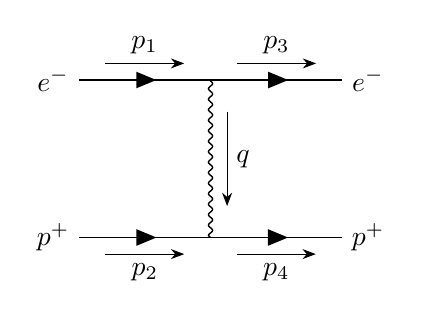
\begin{tikzpicture}
    \begin{feynhand}
      % vertices
      \vertex (e1) at (0,0) {$e^-$};
      \vertex (e2) at (4,0) {$e^-$};
      \vertex (p1) at (0,-2) {$p^+$};
      \vertex (p2) at (4,-2) {$p^+$};
      \vertex  (a) at (2,0);
      \vertex  (b) at (2,-2);
      % particles
      \propag [fer, mom=$p_1$] (e1) to (a);
      \propag [fer, mom=$p_3$] (a) to (e2);
      \propag [fer, mom'=$p_2$] (p1) to (b);
      \propag [fer, mom'=$p_4$] (b) to (p2);
      % boson
      \propag [bos, mom=$q$] (a) to (b);
    \end{feynhand}
  \end{tikzpicture}
  \fi
  \caption{Coulomb Scattering Diagram}
\end{figure}

We are explicitly given the matrix element in chapter 6:
\begin{align*}
  -i\mathcal{M}&=(-ie)(p_1+p_2)^\mu\frac{-ig_{\mu\nu}}{q^2}(+ie)(p_2+p_4)^\nu\\
  q^2&=(p_1-p_3)^2=(p_2-p_4)^2
\end{align*}
And we note that the total cross section is given in the book from equation 6.2:
\begin{align*}
  \sigma(AB\to CD)=&\frac{1}{2E_A}\frac1{2E_B}\frac1{\abs{\vb{v}_A-\vb{v}_B}}\\
  \times&\int\frac{\dd[3]{\vb{p}}_C}{(2\pi)^3}\frac1{2E_C}
  \frac{\dd[3]{\vb{p}}_D}{(2\pi)^3}\frac1{2E_D}\abs{\mathcal{M}}^2
  (2\pi)^4\delta^{(4)}(p_A+p_B-p_C-p_D)
\end{align*}
If we substitute in the process we want to calculate, we have the momenta and energy as prescribed by the diagram:
\begin{align*}
  \sigma({e^-}{p^+}\to {e^-}{p^+})
  =&\frac{1}{2E_1}\frac{1}{2E_2}
  \frac1{\abs{\vb{v}_1-\vb{v}_2}}\\
  \times&\int\frac{\dd[3]{\vb{p}}_{3}}{(2\pi)^3}\frac1{2E_{3}}
  \frac{\dd[3]{\vb{p}}_{4}}{(2\pi)^3}\frac1{2E_{4}}\abs{\mathcal{M}}^2
  (2\pi)^4\delta^{(4)}(p_1+p_2-p_3-p_4)
\end{align*}


\section{A Cross Section}
We want to calculate the invariant matrix element and total cross section for the following:
\begin{figure}[H]
  \centering
  \ifab
    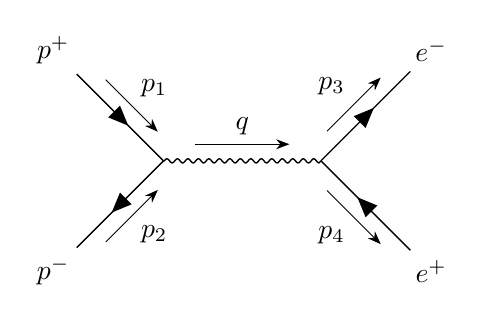
\begin{tikzpicture}
      \begin{feynhand}
        \vertex (p1) at (-1.4, 1.4) {$p^+$};
        \vertex (p2) at (-1.4,-1.4) {$p^-$};
        \vertex (e1) at (3.4, 1.4) {$e^-$};
        \vertex (e2) at (3.4, -1.4) {$e^+$};
        \vertex (a) at (0,0);
        \vertex (b) at (2,0);
        \propag [fer, mom={$p_1$}] (p1) to (a);
        \propag [antfer, mom'={$p_2$}] (p2) to (a);
        \propag [fer, mom={$p_3$}] (b) to (e1);
        \propag [antfer, mom'={$p_4$}] (b) to (e2);
        \propag [bos, mom={$q$}] (a) to (b);
      \end{feynhand}
    \end{tikzpicture}
  \fi
  \caption{Diagram for $p^+p^-\to e^+e^-$}
\end{figure}
Again using the Feynman rules in eq \eqref{eq:fr}

\section{Yukawa Interaction}
Note the Lagrangian we are using is:
\begin{align*}
  \L=-\frac14F'_{\mu\nu}F^{\prime\mu\nu}
  +\frac12\qty[\D_\mu\bar\sigma\D^\mu\bar\sigma]
  +\frac12\qty(\frac{v+\bar\sigma}{v})^2e^2v^2A'_\mu A^{\prime\mu}-V(\bar\sigma)
\end{align*}

\end{document}